\input{../../input/main}

\begin{document}

\begin{center}
  \Large{\textbf{11 класс.}\\
  \textit{29 октября 2014.}}
\end{center}


\begin{center}
  \Large \textbf{Гармонические колебания II.}
\end{center}

\large

\task{ Стеклянная пробирка цилиндрической формы имеет длину $L$ и
  площадь сечения $S$. В неё насыпали немного песка для устойчивости и
  погрузили в воду. Масса пробирки с песком равна $m$. Верхний край
  плавающей пробирки сместили вниз почти до поверхности воды и
  отпустили. Опишите дальнейшее движение пробирки. }
% Туймада, 1.25

\taskpic{ На горизонтальной шероховатой поверхности находится обруч
  радиуса $R$, склеенный из двух однородных половинок массами $m_1$ и
  $m_2$. Определите период малых колебаний обруча вблизи положения
  равновесия. }
{
  \begin{tikzpicture}
    \draw[very thick, interface] (3.8,0) -- (0,0);
    \draw[line width=0.05cm] (3,1) arc (0:-180:1cm)
    node[midway,above,blue] {$m_2$}; 
    \draw[line width=0.02cm] (3,1) arc (0:180:1cm)
    node[midway,below,blue] {$m_{1}$};   
  \end{tikzpicture}
}
% Туймада, 1.31

\task{ Шарик небольших размеров с зарядом $q$ и массой $m$ может
  двигаться без трения по натянутой нити длины $2l$, на концах которой
  закреплены неподвижные заряды $Q$. Найти частоту малых колебаний
  шарика. }
% Паршаков, стр. 118

\task{ По гладкой горизонтальной плоскости со скоростью $v_0$ скользит
  однородный брусок длиной $l$. Брусок наезжает на обширный
  шероховатый участок с коэффициентом трения $\mu$. Через какое время
  брусок остановится? }
% Паршаков, стр. 145

\task{ На горизонтальной плоскости с коэффициентом трения $\mu$ лежит
  брусок массой $m$, соединённый горизонтальной пружиной жёсткостью
  $k$ с вертикальной стенкой. Вначале брусок сместили так, что пружина
  растянулась на $x_0$, и затем отпустили. Через какое время брусок
  остановится, если после его остановки пружина оказалась
  недеформированной? }
% Паршаков, стр. 134

\taskpic{ Вертикально закреплённое кольцо имеет радиус $R$ и толщину
  $h$. В кольцо залита жидкость объёма $V$. Какова частота малых колебаний
  жидкости вокруг положения равновесия?}
{
  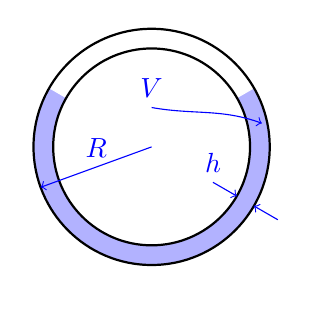
\begin{tikzpicture}
    \draw[fill=blue!30,draw=white] (2,2) ++(30:1.25) -- ++(30:0.25) arc (30:-210:1.5) --
    ++(-30:0.25) arc (-210:30:1.25);
   \draw[thick] (2,2) circle (1.5cm);
   \draw[thick] (2,2) circle (1.25cm);
   \draw[blue,->] (2,2) -- ++(200:1.5cm) node[midway,above] {$R$};
   \draw[blue,->] (2,2)  ++(-30:0.9cm) node[above] {$h$} -- ++(-30:.35cm);
   \draw[blue,->] (2,2) ++(-30:1.85cm) -- ++(-210:.35cm);
   \draw[blue,->] (2,2.5) node[above] {$V$} to[out=-10,in=160] (3.4,2.3);
  \end{tikzpicture}
}

\end{document}


%%% Local Variables: 
%%% mode: latex
%%% TeX-engine:xetex
%%% TeX-PDF-mode: t
%%% End:
